\documentclass{beamer}
\usepackage[utf8]{inputenc}
\usepackage[T1]{fontenc}
\usepackage[brazilian]{babel}
\usepackage{lmodern}
\usetheme{default}
\usecolortheme{beaver}
\usepackage{graphicx,xcolor}
\usepackage{amsmath}


\newtheorem{definicao}[theorem]{Definição}
\newtheorem{teorema}[theorem]{Teorema}
\newtheorem{solucao}[theorem]{Solução}
\beamertemplatenavigationsymbolsempty

\makeatletter
\def\th@mystyle{%
	\ttfamily 
	\setbeamercolor{block title example}{bg=red!30,fg=black}
	\setbeamercolor{block body example}{bg=red!10,fg=black!80}
	\def\inserttheoremblockenv{exampleblock}
}
\makeatother
\theoremstyle{mystyle}
\newtheorem{algoritmo}[theorem]{Algoritmo}

\title{Resolução de Sistemas Lineares - Parte I}
\author
{
	Prof. Jonathan Esteban Arroyo Silva	
}
\institute
{
	Departamento de Ciência da Computação\\
	Universidade Federal de São João del-Rei\\
	\texttt{silva.jea@ufsj.edu.br}
}
\date{}
\logo{
\includegraphics[width=0.2\linewidth]{../ufsj-logo-site}}

\begin{document}
	
\begin{frame}[plain]
    \maketitle
\end{frame}

\begin{frame}[plain]
	\frametitle{Sumário}
	\tableofcontents
\end{frame}

\section{Introdução}

\begin{frame}
	\frametitle{Introdução}
	\begin{itemize}
		\item Uma \textbf{equação} é dita \textbf{linear} se cada termo contém não mais que uma variável e cada variável aparece na primeira potência
		\item Um \textbf{sistema de equações lineares} é um conjunto finito de equações lineares nas mesmas variáveis
	\end{itemize}
\end{frame}

\begin{frame}
	\frametitle{Definição}
	Um sistema de equações lineares $ S $ com $ m $ equações e $ n $ incógnitas é dado por:
	\begin{equation*}
		\left\lbrace 
		\begin{array}{c}
			a_{11}x_{1} + a_{12}x_{2} + \cdots + a_{1n}x_{n} = b_{1}\\
			a_{21}x_{1} + a_{22}x_{2} + \cdots + a_{2n}x_{n} = b_{2}\\
			\vdots\\
			a_{m1}x_{1} + a_{m2}x_{2} + \cdots + a_{mn}x_{n} = b_{m}\\
		\end{array}
		\right. 
	\end{equation*}
	sendo:
	\begin{itemize}
		\item $ a_{ij} \in \mathbb{R} $	os coeficientes
		\item $ b_{i} \in \mathbb{R} $ constantes
		\item $ x_{j} \in \mathbb{R} $ as variáveis (ou incógnitas) do problema
		\item $ i = 1,\ldots, m $ e $ j = 1,\ldots, n $
	\end{itemize}
\end{frame}

\begin{frame}
	\frametitle{Definição II}
	O sistema de equações lineares $ S $ também pode ser escrito na forma matricial como $ \mathbf{Ax} = \mathbf{b}$ ou:
	\begin{equation*}
		\left[
		\begin{array}{cccc}
			a_{11} & a_{12} & \cdots & a_{1n} \\
			a_{21} & a_{22} & \cdots & a_{2n} \\
			\vdots & \vdots & \vdots & \vdots \\
			a_{m1} & a_{m2} & \cdots & a_{mn}\\
		\end{array}
		\right] 
		\begin{bmatrix} x_{1} \\ x_{2} \\ \vdots \\ x_{n} \end{bmatrix}
		=
		\begin{bmatrix} b_{1} \\ b_{2} \\ \vdots \\ b_{m} \end{bmatrix}
	\end{equation*}
\end{frame}

\begin{frame}
	\frametitle{Importância}
	Sistemas de equações lineares aparecem em diferentes problemas das mais diversas áreas da ciência:
	\begin{itemize}
		\item Análise de estruturas
		\item Modelagem de circuitos elétricos
		\item Reações químicas (equilibrar equações)
		\item Programação linear e não-linear
		\item Aprendizagem de máquina (regressão/classificação)
		\item Métodos numéricos
		\begin{itemize}
			\item Interpolação, mínimos quadrados, solução de equações diferenciais
		\end{itemize}
	\end{itemize}
\end{frame}

\begin{frame}
	\frametitle{Classificação dos sistemas}
	Seja um sistema $ \mathbf{Ax} = \mathbf{b}$, com uma matriz quadrada $ \mathbf{A} \in \mathbb{R}^{n\times n} $, tem-se as seguintes possibilidades quanto ao vetor solução \textbf{x}:
	\begin{itemize}
		\item Caso 1: Solução única (consistente e determinado)
		\item Caso 2: Infinitas soluções (consistente e indeterminado)
		\item Caso 3: Nenhuma solução (inconsistente)
	\end{itemize}
\end{frame}

\begin{frame}
	\frametitle{Caso 1 - Exemplo}
	\begin{columns}
		\begin{column}{0.4\textwidth} 
			Seja o sistema $ \mathbf{Ax} = \mathbf{b}$, dado por:
			\begin{equation*}
				\left[
				\begin{array}{cc}
					1 & 1 \\
					1 & -1 
				\end{array}
				\right] 
				\begin{bmatrix} x_{1} \\ x_{2} \end{bmatrix}
				=
				\begin{bmatrix} 3 \\ -1 \end{bmatrix}
			\end{equation*}
			
			O vetor solução é dado por: $ \mathbf{x} = \begin{bmatrix} 1 \\ 2 \end{bmatrix} $
		\end{column}
		\begin{column}{0.6\textwidth}	
			\begin{figure}
				\centering
				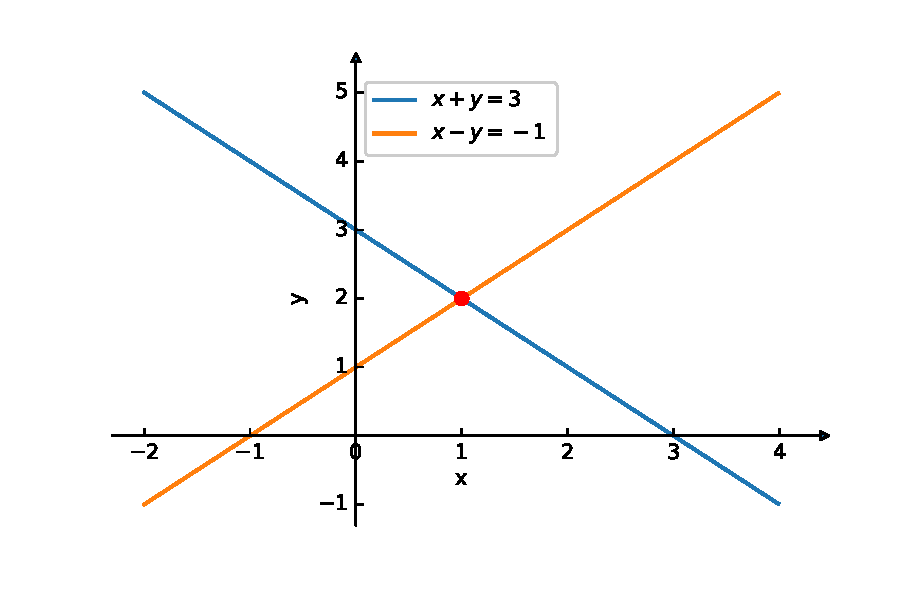
\includegraphics[width=\linewidth]{Figuras/grafico_01}
				\label{fig:grafico_01}
			\end{figure}
		\end{column}
	\end{columns}
\end{frame}

\begin{frame}
	\frametitle{Caso 2 - Exemplo}
	\begin{columns}
		\begin{column}{0.4\textwidth} 
			Seja o sistema $ \mathbf{Ax} = \mathbf{b}$, dado por:
			\begin{equation*}
				\left[
				\begin{array}{cc}
					1 & 1 \\
					2 & 2 
				\end{array}
				\right] 
				\begin{bmatrix} x_{1} \\ x_{2} \end{bmatrix}
				=
				\begin{bmatrix} 1 \\ 2 \end{bmatrix}
			\end{equation*}
			
			O vetor solução é dado por: $ \mathbf{x} = \begin{bmatrix} 1 - \lambda \\ \lambda \end{bmatrix} $, sendo $ \lambda \in \mathbb{R} $
		\end{column}
		\begin{column}{0.6\textwidth}	
			\begin{figure}
				\centering
				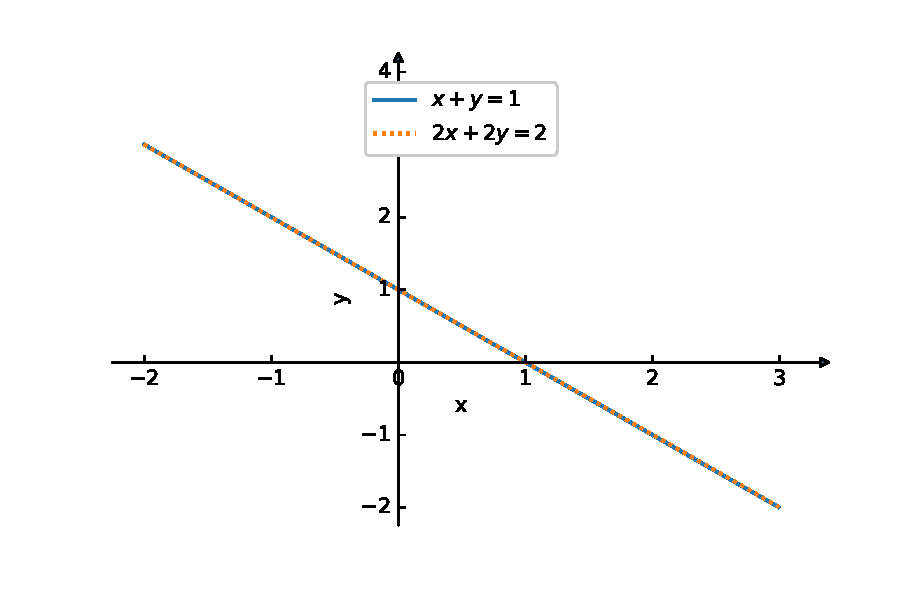
\includegraphics[width=\linewidth]{Figuras/grafico_02}
				\label{fig:grafico_02}
			\end{figure}
		\end{column}
	\end{columns}
\end{frame}

\begin{frame}
	\frametitle{Caso 3 - Exemplo}
	\begin{columns}
		\begin{column}{0.4\textwidth} 
			Seja o sistema $ \mathbf{Ax} = \mathbf{b}$, dado por:
			\begin{equation*}
				\left[
				\begin{array}{cc}
					1 & 1 \\
					1 & 1 
				\end{array}
				\right] 
				\begin{bmatrix} x_{1} \\ x_{2} \end{bmatrix}
				=
				\begin{bmatrix} 1 \\ 4 \end{bmatrix}
			\end{equation*}
			
			Não existe \textbf{x} que satisfaça $ \mathbf{Ax} = \mathbf{b}$
		\end{column}
		\begin{column}{0.6\textwidth}	
			\begin{figure}
				\centering
				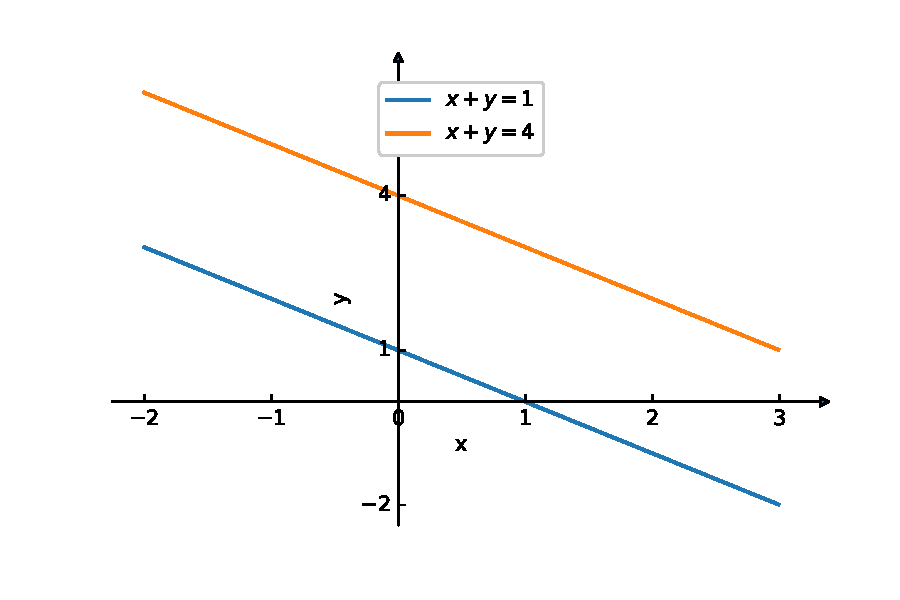
\includegraphics[width=\linewidth]{Figuras/grafico_03}
				\label{fig:grafico_03}
			\end{figure}
		\end{column}
	\end{columns}
\end{frame}

\begin{frame}
	\frametitle{Existência e Unicidade de solução}
	Seja uma matriz quadrada $ \mathbf{A} \in \mathbb{R}^{n\times n} $, as seguintes afirmações são equivalentes:
	\begin{itemize}
		\item $ \mathbf{A}^{-1} $ existe
		\item A única solução para o sistema homogêneo $ \mathbf{Ay} = \mathbf{0}$ é se $ \mathbf{y} = \mathbf{0} $
		\item O posto da matriz $ \mathbf{A} $ é $ n $
		\item $\det (\mathbf{A}) \neq 0$
		\item Dado qualquer vetor $ \mathbf{b} $, existe exatamente um vetor $ \mathbf{x} $ que satisfaça $ \mathbf{Ax} = \mathbf{b}$
	\end{itemize}
\end{frame}

\begin{frame}
	\frametitle{Exemplo}
	Verifique se os exemplos anteriores possuem solução através do cálculo do determinante:
	\pause
	\begin{itemize}
		\item Exemplo 1: como o determinante de $ \mathbf{A} = \left[
		\begin{array}{cc}
			1 & 1 \\
			1 & -1 
		\end{array}
		\right] $ é igual a $ 2 \neq 0 $, então \textbf{existe solução} e é \textbf{única}
		\item Exemplo 2: como o determinante de $ \mathbf{A} = \left[
		\begin{array}{cc}
			1 & 1 \\
			2 & 2 
		\end{array}
		\right] $ é igual a 0, então o sistema não tem solução ou a \textbf{solução não é única}
		\item Exemplo 3: como o determinante de $ \mathbf{A} = \left[
		\begin{array}{cc}
			1 & 1 \\
			1 & 1 
		\end{array}
		\right] $ é igual a 0, então o sistema \textbf{não tem solução} ou a solução não é única
	\end{itemize}
\end{frame}

\begin{frame}
	\frametitle{Classificação dos Métodos Numéricos}
	A partir deste ponto, considera-se que \textbf{A} é uma matriz quadrada e não-singular (tem inversa). Sendo assim, os métodos que serão apresentados podem ser divididos em:
	\begin{itemize}
		\item Métodos diretos: Fornecem a solução exata do problema, a menos de erros de arredondamento, após um número finito de operações
		\item Métodos iterativos: Geram uma sequência de vetores a partir de uma aproximação inicial e, sob certas condições, essa sequência converge para a solução do problema	 
	\end{itemize}
\end{frame}

\section{Métodos Diretos}

\begin{frame}
	\frametitle{Métodos Diretos - Introdução}
	É chamado de \textbf{sistema triangular inferior} \textbf{L} de ordem $ n $ o sistema da forma:
	\begin{equation*}
		\left[
		\begin{array}{ccccc}
			l_{11} &   0    &    0   & \cdots & 0 \\
			l_{21} & l_{22} &    0   & \cdots & 0 \\
			\vdots & \vdots & \vdots & \ddots & \vdots \\
			l_{n1} & l_{n2} & l_{n3} & \cdots & l_{nn}\\
		\end{array}
		\right] 
		\begin{bmatrix} x_{1} \\ x_{2} \\ \vdots \\ x_{n} \end{bmatrix}
		=
		\begin{bmatrix} b_{1} \\ b_{2} \\ \vdots \\ b_{n} \end{bmatrix}
	\end{equation*}
	\pause
	Um \textbf{sistema triangular superior} \textbf{U} de ordem $ n $ é dado de forma análoga.
\end{frame}

\begin{frame}
	\frametitle{Substituição - I}
	A resolução de um sistema desta forma é dado pelo procedimento chamado de \textbf{substituição} ou substituições sucessivas:
	\begin{gather*}
		\alert{l_{11}}x_{1} = \alert{b_{1}} \Rightarrow x_{1} = \alert{b_{1}/l_{11}}\\
		\alert{l_{21}x_{1}} + \alert{l_{22}}x_{2} = \alert{b_{2}} \Rightarrow x_{2} = \alert{(b_{2} - l_{21}x_{1})/l_{22}}\\
		\vdots\\
		\alert{l_{n1}x_{1}} + \alert{l_{n2}x_{2}} + \ldots + \alert{l_{n2}}x_{n} = \alert{b_{n}} \Rightarrow\\
		x_{n} = \alert{(b_{n} - l_{n1}x_{1} - l_{n2}x_{2} - \ldots - l_{n,n-1}x_{n-1})/l_{nn}}
	\end{gather*}
	Sendo os valores em vermelho ou dados ou calculados ao longo do processo.
\end{frame}

\begin{frame}
	\frametitle{Substituição - II}
	Outra forma de apresentar a resolução por substituição é a seguinte:
	\begin{equation*}
		x_{i} = \left(b_{i} - \sum_{j=1}^{i-1} l_{ij} x_{j} \right) / l_{ii}, \;\;\; i = 1,\ldots, n
	\end{equation*}
	sendo o lado direito composto com valores dados ou calculados ao longo do processo.
\end{frame}

\begin{frame}
	\frametitle{Substituição - Exemplo}
	Resolva o seguinte sistema triangular inferior:
	\begin{equation*}
		\left[
		\begin{array}{cccc}
			2 & 0 & 0 & 0 \\
			3 & 5 & 0 & 0 \\
			1 & -6 & 8 & 0 \\
			-1 & 4 & -3 & 9 \\
		\end{array}
		\right] 
		\begin{bmatrix} x_{1} \\ x_{2} \\ x_{3} \\ x_{4} \end{bmatrix}
		=
		\begin{bmatrix} 4 \\ 1 \\ 48 \\ 0 \end{bmatrix}
	\end{equation*}
	\pause 
	Solução:
	\begin{gather*}
		\alert{2}x_{1} = \alert{4} \Rightarrow x_{1} = \alert{4/2} = \alert{2}\\
		\alert{3x_{1}} + \alert{5}x_{2} = \alert{1} \Rightarrow x_{2} = \alert{(1 - 3\cdot2)/5} = \alert{-1}\\
		\alert{x_{1}} \alert{- 6x_{2}} + \alert{8}x_{3} = \alert{54} \Rightarrow x_{3} = \alert{(48 - 2 - (-6)\cdot (-1))/8} = \alert{5}\\
		\alert{-x_{1}} + \alert{4x_{2}} \alert{-3x_{3}} + \alert{9}x_{4} = \alert{0} \Rightarrow\\
		x_{4} = \alert{(-(-1)\cdot2 - 4\cdot(-1)  - (-3)\cdot 5)/9} = \alert{21/9} = \alert{7/3}
	\end{gather*}
\end{frame}

\begin{frame}
	\frametitle{Substituição - III}
	Assim, dada a matriz \textbf{L} e o vetor \textbf{b}, o algoritmo do procedimento de substituição pode ser descrito como:
	\begin{algoritmo}
		x$ _{\texttt{1}}$ $\leftarrow$ b$ _{\texttt{1}}$/L$ _{\texttt{11}}$\\
		soma $\leftarrow$ 0\\
		Para i = 2,$\ldots$,n, faça:\\
		\quad soma $\leftarrow$ b$ _{\texttt{i}}$\\
		\quad Para j = 1,$\ldots$,i-1, faça:\\
		\quad\quad soma $\leftarrow$ soma - L$ _{\texttt{ij}}$ * x$ _{\texttt{j}} $ \\
		\quad x$ _{\texttt{i}} \leftarrow$ soma/L$ _{\texttt{ii}}$
	\end{algoritmo}
\end{frame}

\begin{frame}
	\frametitle{Retro-substituição}
	De forma análoga, dado um \textbf{sistema triangular superior} com uma matriz \textbf{U} e vetor \textbf{b}, o algoritmo do procedimento de retro-substituição pode ser descrito como:
	\begin{algoritmo}
		x$ _{\texttt{n}}$ $\leftarrow$ b$ _{\texttt{n}}$/L$ _{\texttt{nn}}$\\
		soma $\leftarrow$ 0\\
		Para i = n-1,$\ldots$,1, faça:\\
		\quad soma $\leftarrow$ b$ _{\texttt{i}}$\\
		\quad Para j = i+1,$\ldots$,n, faça:\\
		\quad\quad soma $\leftarrow$ soma - L$ _{\texttt{ij}}$ * x$ _{\texttt{j}} $ \\
		\quad x$ _{\texttt{i}} \leftarrow$ soma/U$ _{\texttt{ii}}$
	\end{algoritmo}
\end{frame}

\subsection{Eliminação Gaussiana}

\begin{frame}
	\frametitle{Método de Eliminação Gaussiana}
	 A ideia fundamental do método é transformar a matriz \textbf{A} numa matriz triangular superior utilizando \textbf{operações elementares} sobre as linhas da matriz original, para em seguida usar a retro-substituição
	\begin{itemize}
		\item Mais precisamente, utilizaremos a operação que consiste em substituir uma equação (linha da matriz) pela diferença entre essa mesma equação e uma outra equação multiplicada por uma \alert{constante} diferente de zero
		\item Tal operação não altera a solução do sistema, isto é, obtêm-se com ela outro sistema equivalente ao original (desde que aplicado a todo o sistema)
		\item Para isso utilizaremos o conceito de \textbf{matriz estendida} (ou aumentada)
	\end{itemize}
\end{frame}

\begin{frame}
	\frametitle{Método de Eliminação Gaussiana - Exemplo}
	 Seja o sistema
	 \begin{equation*}
	 	\left[
	 	\begin{array}{ccc}
	 		2 & 1 & 1  \\
	 		4 & -6 & 0  \\
	 		-2 & 7 & 2
	 	\end{array}
	 	\right] 
	 	\begin{bmatrix} x_{1} \\ x_{2} \\ x_{3} \end{bmatrix}
	 	=
	 	\begin{bmatrix} 26 \\ 7 \\ 91 \end{bmatrix}
	\end{equation*}
	aplique o método de Eliminação Gaussiana.

\end{frame}

\begin{frame}
	\frametitle{Método de Eliminação Gaussiana - Exemplo}
	\textbf{Passo 1:} Montar a matriz estendida
	\begin{equation*}
		\left[
		\begin{array}{ccc|c}
			2  & 1  & 1 & 26 \\
			4  & -6 & 0 & 7  \\
			-2 & 7  & 2 & 91
		\end{array}
		\right]
	\end{equation*}

	\textbf{Passo 2:} Calcular as \alert{constantes} para aplicar as operações elementares
	\begin{gather*}
		m_{21} = \dfrac{a_{21}}{a_{11}} = 4/2 = 2\\
		m_{31} = \dfrac{a_{31}}{a_{11}} = -2/2 = -1
	\end{gather*}
\end{frame}

\begin{frame}
	\frametitle{Método de Eliminação Gaussiana - Exemplo}
	\textbf{Passo 3:} Aplicar as operações elementares nas respectivas linhas
	\begin{gather*}
		L_{2} \leftarrow L_{2} - m_{21}\cdot L_{1} = L_{2} - 2\cdot L_{1}\\
		L_{3} \leftarrow L_{3} - m_{31}\cdot L_{1} = L_{3} + 1\cdot L_{1}
	\end{gather*}

	Resultando no seguinte sistema:
	\begin{equation*}
		\left[
		\begin{array}{ccc|c}
			2  & 1  & 1 & 26 \\
			0  & -8 & -2 & -45  \\
			0  &  8 & 3 & 117
		\end{array}
		\right]
	\end{equation*}
\end{frame}

\begin{frame}
	\frametitle{Método de Eliminação Gaussiana - Exemplo}
	\textbf{Passo 4:} Repetir o \textbf{Passo 2} na próxima coluna
	\begin{equation*}
		m_{32} = \dfrac{a_{32}}{a_{22}} = 8/(-8) = -1
	\end{equation*}
	
	\textbf{Passo 5:} Repetir o \textbf{Passo 3} nas respectivas linhas
	\begin{equation*}
		L_{3} \leftarrow L_{3} - m_{32}\cdot L_{2} = L_{3} + 1\cdot L_{2}
	\end{equation*}
	
	Resultando no seguinte sistema:
	\begin{equation*}
		\left[
		\begin{array}{ccc|c}
			2  & 1  & 1 & 26 \\
			0  & -8 & -2 & -45  \\
			0  &  0 & 1 & 72
		\end{array}
		\right]
	\end{equation*}
\end{frame}

\begin{frame}
	\frametitle{Método de Eliminação Gaussiana}
	Ao utilizar apenas \textbf{operações elementares} foi possível chegar a um sistema equivalente ao original, que é possível de resolver facilmente por retro-substituição, como comentado anteriormente.
\end{frame}

\subsection{Decomposição LU}

\begin{frame}
	\frametitle{Decomposição LU}
	A ideia fundamental do método é que uma matriz quadrada pode ser escrita como o produto de duas matrizes \textbf{L} e \textbf{U}, respectivamente, uma matriz triangular inferior e superior. Ou seja, a matriz original \textbf{A} pode ser escrita como:
	\begin{equation*}
		\mathbf{A} = \mathbf{LU}
	\end{equation*}
	
	Assim, podemos reescrever o sistema da seguinte forma:
	\begin{equation}\label{equacao_1}
		\mathbf{Ax} = \mathbf{b} \rightarrow \mathbf{LUx} = \mathbf{b}
	\end{equation}
\end{frame}

\begin{frame}
	\frametitle{Decomposição LU}
	Supondo que $ \mathbf{Ux} = \mathbf{y} $, um vetor \textbf{y} que neste momento não conheço (vetor de incógnitas), da equação \ref{equacao_1} podemos escrever:
	\begin{equation*}
		\mathbf{Ly} = \mathbf{b}
	\end{equation*}
	e resolver o sistema para encontrar \textbf{y}. 
	
	Ao saber os valores de \textbf{y}, será possível resolver o sistema:
	\begin{equation*}
		\mathbf{Ux} = \mathbf{y}
	\end{equation*}
	e encontrar os valores para \textbf{x}.
\end{frame}

\begin{frame}
	\frametitle{Decomposição LU - Detalhes}
	\begin{itemize}
		\item Como \textbf{L} é triangular inferior podemos resolver $ \mathbf{Ly} = \mathbf{b} $ facilmente usando o algoritmo de substituição
		\item  Como \textbf{U} é uma matriz triangular superior, podemos resolver este sistema usando o algoritmo da retro-substituição
	\end{itemize}
\end{frame}

\begin{frame}
	\frametitle{Decomposição LU - Condição de existência}
	Seja \textbf{A} uma matriz quadrada de ordem $ n $ e $ \mathbf{A}_{k} $ o \textit{menor	principal}, composto das $ k $ primeiras linhas e $ k $ primeiras colunas de \textbf{A}. Se $ \det(\mathbf{A}_{k})\neq 0 $ para $ k = 1, 2, \ldots , n - 1 $. Então existe:
	\begin{itemize}
		\item uma \textbf{única} matriz triangular inferior $ \mathbf{L} = (l_{ij})$ com $ l_{ii} = 1 $, para $ i = 1, \ldots , n $
		\item  uma \textbf{única} matriz triangular superior $ \mathbf{U} = (u_{ij})$
	\end{itemize}
	De forma que $ \mathbf{A} = \mathbf{LU} $, além disso, $ \det(\mathbf{A}) = u_{11}u_{22}\ldots u_{nn} $
\end{frame}

\begin{frame}
	\frametitle{Decomposição LU - Montagem de L e U}
	Como visto em \textit{Álgebra linear}, as \textbf{operações elementares} podem ser vistas como matrizes. Tendo isso em mente, faremos o exemplo anterior novamente.
	
	Seja o sistema:
	\begin{equation*}
		\left[
		\begin{array}{ccc}
			2 & 1 & 1  \\
			4 & -6 & 0  \\
			-2 & 7 & 2
		\end{array}
		\right] 
		\begin{bmatrix} x_{1} \\ x_{2} \\ x_{3} \end{bmatrix}
		=
		\begin{bmatrix} 26 \\ 7 \\ 91 \end{bmatrix}
	\end{equation*}
	aplique o método de Eliminação Gaussiana.
\end{frame}

\begin{frame}
	\frametitle{Decomposição LU - Montagem de L e U}
	Como trabalharemos com matrizes não é necessário montar a matriz estendida, assim, podemos pular o \textbf{Passo 1} do método anterior.

	\textbf{Passo 1:} Calcular as \alert{constantes} para aplicar as operações elementares
	\begin{gather*}
		m_{21} = 2\\
		m_{31} = -1
	\end{gather*}

	\textbf{Passo 2:} Montar a matriz de operações elementares utilizando as \alert{constantes} calculadas no passo anterior
	\begin{equation*}
		\mathbf{M}_{1} =
		\left[
		\begin{array}{ccc}
			1 & 0 & 0  \\
			-m_{21} & 1 & 0  \\
			-m_{31} & 0 & 1
		\end{array}
		\right] 
		 =
		\left[
		\begin{array}{ccc}
			1 & 0 & 0  \\
			-2 & 1 & 0  \\
		   1 & 0 & 1
		\end{array}
		\right]
	\end{equation*}
\end{frame}

\begin{frame}
	\frametitle{Decomposição LU - Montagem de L e U}
	\textbf{Passo 3:} Multiplicar a matriz de operações elementares nos dois lados da igualdade pelo lado esquerdo
	\begin{gather*}
		\mathbf{M}_{1}\mathbf{Ax} = \mathbf{M}_{1}\mathbf{b}\\
		\left[
		\begin{array}{ccc}
			1 & 0 & 0  \\
			-2 & 1 & 0  \\
			1 & 0 & 1
		\end{array}
		\right]
		\left[
		\begin{array}{ccc}
			2 & 1 & 1  \\
			4 & -6 & 0  \\
			-2 & 7 & 2
		\end{array}
		\right] 
		\begin{bmatrix} x_{1} \\ x_{2} \\ x_{3} \end{bmatrix}
		=
		\left[
		\begin{array}{ccc}
			1 & 0 & 0  \\
			-2 & 1 & 0  \\
			1 & 0 & 1
		\end{array}
		\right]
		\begin{bmatrix} 26 \\ 7 \\ 91 \end{bmatrix}\\
		\left[
		\begin{array}{ccc}
			2 & 1 & 1  \\
			0 & -8 & -2  \\
			0 & 8 & 3
		\end{array}
		\right] 
		\begin{bmatrix} x_{1} \\ x_{2} \\ x_{3} \end{bmatrix}
		=
		\begin{bmatrix} 26 \\ -45 \\ 117 \end{bmatrix}
	\end{gather*}
\end{frame}

\begin{frame}
	\frametitle{Decomposição LU - Montagem de L e U}
	Repare na semelhança entre os resultados parciais de ambas as abordagens.
	
	\textbf{Passo 4:} Repetir o \textbf{Passo 1} para a próxima coluna
	\begin{equation*}
		m_{32} = -1
	\end{equation*}
	
	\textbf{Passo 5:} Repetir o \textbf{Passo 2} utilizando as novas \alert{constantes}
	\begin{equation*}
		\mathbf{M}_{2} =
		\left[
		\begin{array}{ccc}
			1 & 0 & 0  \\
			0 & 1 & 0  \\
			0 & -m_{32} & 1
		\end{array}
		\right] 
		=
		\left[
		\begin{array}{ccc}
			1 & 0 & 0  \\
			0 & 1 & 0  \\
			0 & 1 & 1
		\end{array}
		\right]
	\end{equation*}
\end{frame}

\begin{frame}
	\frametitle{Decomposição LU - Montagem de L e U}
	\textbf{Passo 6:} Multiplicar a matriz de operações elementares nos dois lados da igualdade pelo lado esquerdo
	\begin{gather*}
		\mathbf{M}_{2}\mathbf{M}_{1}\mathbf{Ax} = \mathbf{M}_{2}\mathbf{M}_{1}\mathbf{b}\\
		\left[
		\begin{array}{ccc}
			1 & 0 & 0  \\
			0 & 1 & 0  \\
			0 & 1 & 1
		\end{array}
		\right]
		\left[
		\begin{array}{ccc}
			2 & 1 & 1  \\
			0 & -8 & -2  \\
			0 & 8 & 3
		\end{array}
		\right] 
		\begin{bmatrix} x_{1} \\ x_{2} \\ x_{3} \end{bmatrix}
		=
		\left[
		\begin{array}{ccc}
			1 & 0 & 0  \\
			0 & 1 & 0  \\
			0 & 1 & 1
		\end{array}
		\right]
		\begin{bmatrix} 26 \\ -45 \\ 117 \end{bmatrix}\\
		\left[
		\begin{array}{ccc}
			2 & 1 & 1  \\
			0 & -8 & -2  \\
			0 & 0 & 1
		\end{array}
		\right] 
		\begin{bmatrix} x_{1} \\ x_{2} \\ x_{3} \end{bmatrix}
		=
		\begin{bmatrix} 26 \\ -45 \\ 72 \end{bmatrix}
	\end{gather*}
\end{frame}

\begin{frame}
	\frametitle{Decomposição LU - Montagem de L e U}
	Após o último passo chegamos na matriz triangular superior desejada, ou seja:
	\begin{equation*}
		\mathbf{M}_{2}\mathbf{M}_{1}\mathbf{A} = \textbf{U}
	\end{equation*}

	Chamando $ \mathbf{M}_{2}\mathbf{M}_{1} = \mathbf{M} $, teremos:
	\begin{equation*}
		\mathbf{M}\mathbf{A} = \textbf{U} \rightarrow \mathbf{A} =  \mathbf{M}^{-1}\textbf{U} 
	\end{equation*}
	pela \textbf{condição de existência} das matrizes \textbf{L} e \textbf{U}, elas são únicas, logo, chamando $ \mathbf{M}^{-1} = \mathbf{L} $, teremos:
	\begin{equation*}
		\mathbf{A} =  \mathbf{L}\textbf{U} 
	\end{equation*}

	Para maiores detalhes ler \emph{Michael T. Heath. Scientific Computing. An Introductory Survey (2018). pags. 65-68}.
\end{frame}

\begin{frame}
	\frametitle{Decomposição LU - Montagem de L e U}
	Tudo isso para mostrar que:
	\begin{gather*}
		\mathbf{A} = \mathbf{L}\mathbf{U}\\
		\left[
		\begin{array}{ccc}
			2 & 1 & 1  \\
			4 & -6 & 0  \\
			-2 & 7 & 2
		\end{array}
		\right] 
		=
		\left[
		\begin{array}{ccc}
			1 & 0 & 0  \\
			m_{21} & 1 & 0  \\
			m_{31} & m_{32} & 1
		\end{array}
		\right]
		\left[
		\begin{array}{ccc}
			2 & 1 & 1  \\
			0 & -8 & -2  \\
			0 & 0 & 1
		\end{array}
		\right]\\ 
		\left[
		\begin{array}{ccc}
			2 & 1 & 1  \\
			4 & -6 & 0  \\
			-2 & 7 & 2
		\end{array}
		\right] 
		=
		\left[
		\begin{array}{ccc}
			1 & 0 & 0  \\
			2 & 1 & 0  \\
			-1 & -1 & 1
		\end{array}
		\right]
		\left[
		\begin{array}{ccc}
			2 & 1 & 1  \\
			0 & -8 & -2  \\
			0 & 0 & 1
		\end{array}
		\right]
	\end{gather*}
	Assim, é possível montar as matrizes da \textbf{Decomposição LU} através do \textbf{Método de eliminação gaussiana} (sem utilizar o conceito de matriz estendida).
\end{frame}

\begin{frame}
	\frametitle{Decomposição LU - Mais detalhes}
	A decomposição LU entretanto é importante do ponto de vista computacional, uma vez que é normal acontecerem problemas matemáticos onde apenas o vetor \textbf{b} muda de valores e a matriz \textbf{A} se mantém fixa.
	Logo, tendo realizado previamente a decomposição de \textbf{A} em \textbf{L} e \textbf{U}, precisaríamos apenas resolver:
	\begin{equation*}
		\mathbf{Ly} = \mathbf{b}
	\end{equation*}
	e em seguida: 
	\begin{equation*}
		\mathbf{Ux} = \mathbf{y}
	\end{equation*}
	para encontrar \textbf{x}, ao invés de ter que transformar a matriz \textbf{A} em triangular toda vez que mudamos o vetor \textbf{b}.
\end{frame}

\begin{frame}
	\frametitle{Decomposição LU - Eliminação gaussiana}
	Inicializando as matrizes \textbf{L} e \textbf{U} como matrizes identidade e copia da matriz \textbf{A}, respectivamente, teremos:
	\begin{algoritmo}
		Para k = 1,$\ldots$,n-1, faça:\\
		\quad Se U$_{\texttt{kk}}$ == 0 faça:\\
		\quad\quad \alert{BREAK}\\
		\quad Para i = k+1,$\ldots$,n, faça:\\
		\quad\quad L$ _{\texttt{ik}} \leftarrow$ U$ _{\texttt{ik}}/$ U$ _{\texttt{kk}}$\\
		\quad Para j = k,$\ldots$,n, faça:\\
		\quad\quad Para i = k+1,$\ldots$,n, faça:\\
		\quad\quad\quad U$ _{\texttt{ij}} \leftarrow$ U$ _{\texttt{ij}}$-L$ _{\texttt{ik}}$*U$ _{\texttt{kj}}$
	\end{algoritmo}
\end{frame}

\begin{frame}
	\frametitle{Exemplo - Implementação}
	\centering
	\href{https://colab.research.google.com/drive/1hzQL6xUVDv2JrtFvoZnO_3NGbbaRZecC?usp=sharing}{\beamergotobutton{Link para exemplo interativo}}
\end{frame}

\begin{frame}
	\frametitle{Conclusão I}	
	Foram abordados os seguintes assuntos:
	\begin{itemize}
		\item Definição de sistema linear e a sua importância na ciência
		\item Classificação dos sistemas lineares: solução única, infinitas soluções, nenhuma solução
		\item Existência e unicidade da solução
	\end{itemize}
\end{frame}

\begin{frame}
	\frametitle{Conclusão II}	
	\begin{itemize}
		\item Classificação dos métodos numéricos para resolver este tipo de problema: métodos diretos e métodos iterativos
		\item Introdução aos métodos diretos 
		\item Sistemas triangulares, inferior e superior, assim como a sua resolução por substituição e retro-substituição respectivamente
	\end{itemize}
\end{frame}

\begin{frame}
	\frametitle{Conclusão III}	
	\begin{itemize}
		\item Método de eliminação gaussiana utilizando matriz estendida
		\item Conceito de decomposição LU, condição de existência
		\item Montagem das matrizes \textbf{L} e \textbf{U} através do método de eliminação gaussiana
	\end{itemize}
\end{frame}

\begin{frame}[plain]
\bigskip
\bigskip
\bigskip
\bigskip
\bigskip
\begin{figure}
	\centering
	
\includegraphics[width=0.9\linewidth]{../krillin_v}
	\label{fig:luffyv}
\end{figure}
\end{frame}

\end{document}
